% Drawing 74/02-2 -- folder 74, batch 02, archive page 22 (PDF page 23).
% Transcription: deux versions d'un même schéma. En haut, trois blocs de symboles reliés par des faisceaux de traits croisés. Le premier bloc, surmonté de « $\{1,2,3\} = I_3$ », porte les trois lignes $\xi_1\ \xi_2\ \xi_3$ / $\hat\xi_1\ \hat\xi_2\ \hat\xi_3$ / $\xi_{23}\ \xi_{31}\ \xi_{12}$ ; le deuxième, surmonté de « $\{4,5,6\} =$ » et d'un symbole encadré $\tau_3$, porte $\xi_4\ \xi_5\ \xi_6$ / $\hat\xi_4\ \hat\xi_5\ \hat\xi_6$ / $\xi_{56}\ \xi_{64}\ \xi_{45}$, avec en regard l'accolade « $I_1 = \{$\ill{}$, *, !\}$ » ; le troisième, en bas, porte $\xi_{14}\ \xi_{15}\ \xi_{16}$ / $\xi_{24}\ \xi_{25}\ \xi_{26}$ / $\xi_{34}\ \xi_{35}\ \xi_{36}$, avec « $\{1,2,3\} = I_3$ » à droite, « $\{4,5,6\}$ » au-dessous et un \uncertain{$\tau_3$} cerclé. À droite, un triangle dont les trois sommets portent chacun un des trois blocs, marqué « I ». En bas de page, le même schéma redessiné : le bloc $\xi_1 \ldots \xi_{12}$ relié d'un côté au bloc $\xi_{4} \ldots \xi_{45}$, de l'autre au bloc $\xi_{14} \ldots \xi_{36}$.
% Kind: schema of blocks joined by bundles of lines (two versions). Method 2 (schematic redraw from the facsimile). Status: partial.
% Notes: Top: block xi1..xi12 under {1,2,3} = I_3, block xi4..xi45 under {4,5,6} = with a boxed tau_3 and the brace I_1 = {?, *, !}, block xi14..xi36 with {1,2,3} = I_3, {4,5,6} under it and a circled tau_3; bundles of crossed strokes join the blocks (each bundle drawn as a few representative strokes, not stroke for stroke). Right: the small triangle with a block at each corner, drawn as its outline only (its tiny labels are illegible at this size; the label I was not found in the crop). Bottom: the schema redrawn, block xi1.. joined to xi4.. and to xi14...
% Coordinates: 1 unit = 1 mm = 1/100 of the crop width (bbox in page fractions: [0.12, 0.05, 0.75, 0.67]).
% Redrawn by Claude (claude-opus-5-5), issue #73, 2026-11-07; not checked by a human; not compiled (no TeX in the session).
% Rights: reproduces part of the work -- behind RENDER_TRANSCRIPTS, never published by itself.
\documentclass[tikz,border=3pt]{standalone}
\usepackage{amsmath,amssymb}
\usetikzlibrary{patterns,arrows.meta}
\tikzset{pencil/.style={black!45}, struck/.style={black!35}, mark/.style={circle,draw,inner sep=1.3pt}, pt/.style={circle,fill,inner sep=0.9pt}, opt/.style={circle,draw,fill=white,inner sep=1.1pt}}
\begin{document}
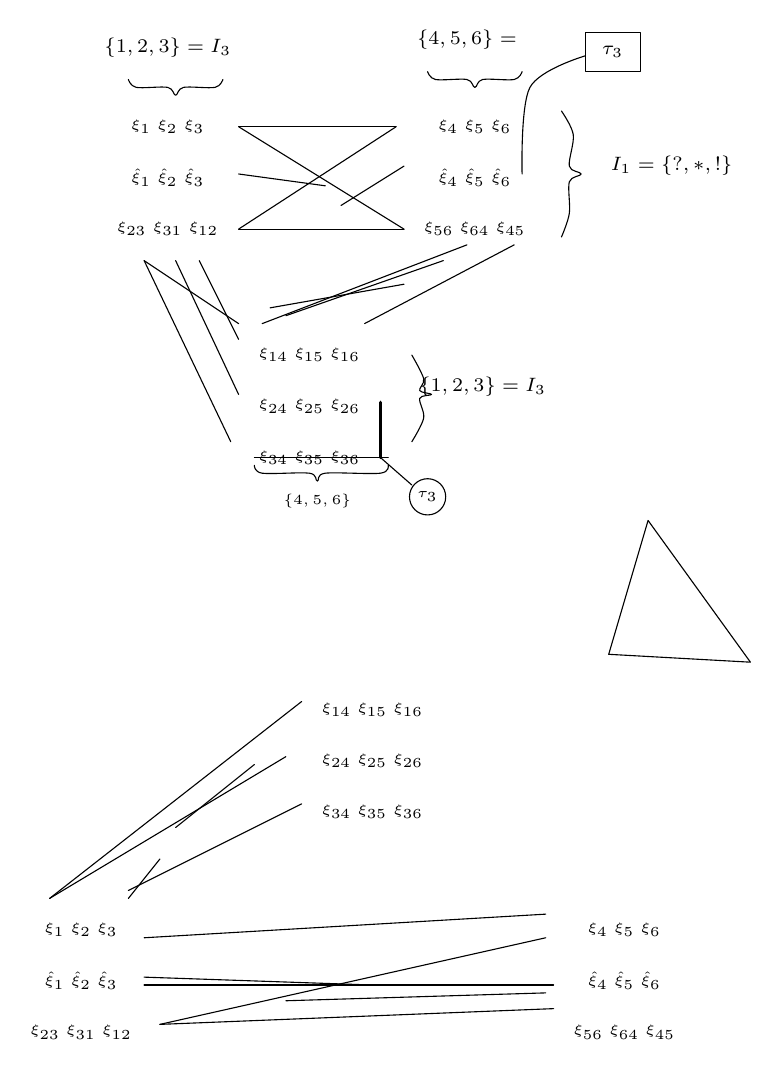
\begin{tikzpicture}[x=1mm,y=1mm,line cap=round,line join=round,font=\scriptsize]
\node[inner sep=1pt] at (25,-7) {\scriptsize $\{1,2,3\}=I_3$};
\draw plot[smooth, tension=0.55] coordinates {(20,-11) (21,-12) (25,-12) (26,-13) (27,-12) (31,-12) (32,-11)};
\node[inner sep=1pt] at (25,-17) {\tiny $\xi_1\ \xi_2\ \xi_3$};
\node[inner sep=1pt] at (25,-23.5) {\tiny $\hat\xi_1\ \hat\xi_2\ \hat\xi_3$};
\node[inner sep=1pt] at (25,-30) {\tiny $\xi_{23}\ \xi_{31}\ \xi_{12}$};
\node[inner sep=1pt] at (63,-6) {\scriptsize $\{4,5,6\}=$};
\draw plot[smooth, tension=0.55] coordinates {(58,-10) (59,-11) (63,-11) (64,-12) (65,-11) (69,-11) (70,-10)};
\draw (78,-5) -- (85,-5) -- (85,-10) -- (78,-10) -- cycle;
\node[inner sep=1pt] at (81.5,-7.5) {\scriptsize $\tau_3$};
\draw plot[smooth, tension=0.55] coordinates {(70,-23) (71,-12) (78,-8)};
\node[inner sep=1pt] at (64,-17) {\tiny $\xi_4\ \xi_5\ \xi_6$};
\node[inner sep=1pt] at (64,-23.5) {\tiny $\hat\xi_4\ \hat\xi_5\ \hat\xi_6$};
\node[inner sep=1pt] at (64,-30) {\tiny $\xi_{56}\ \xi_{64}\ \xi_{45}$};
\draw plot[smooth, tension=0.55] coordinates {(75,-15) (76.5,-18) (76,-22) (77.5,-23) (76,-24) (76,-28) (75,-31)};
\node[inner sep=1pt] at (89,-22) {\scriptsize $I_1=\{?,*,!\}$};
\draw (34,-17) -- (54,-17);
\draw (34,-17) -- (55,-30);
\draw (34,-30) -- (54,-17);
\draw (34,-30) -- (55,-30);
\draw (34,-23) -- (45,-24.5);
\draw (47,-27) -- (55,-22);
\draw (22,-34) -- (34,-42);
\draw (22,-34) -- (33,-57);
\draw (26,-34) -- (34,-51);
\draw (29,-34) -- (34,-44);
\draw (37,-42) -- (63,-32);
\draw (40,-41) -- (60,-34);
\draw (50,-42) -- (69,-32);
\draw (38,-40) -- (55,-37);
\node[inner sep=1pt] at (43,-46) {\tiny $\xi_{14}\ \xi_{15}\ \xi_{16}$};
\node[inner sep=1pt] at (43,-52.5) {\tiny $\xi_{24}\ \xi_{25}\ \xi_{26}$};
\node[inner sep=1pt] at (43,-59) {\tiny $\xi_{34}\ \xi_{35}\ \xi_{36}$};
\draw plot[smooth, tension=0.55] coordinates {(56,-46) (57.5,-49) (57,-50.5) (58.5,-51) (57,-51.5) (57.5,-54) (56,-57)};
\node[inner sep=1pt] at (65,-50) {\scriptsize $\{1,2,3\}=I_3$};
\draw[very thick] (52,-52) -- (52,-59);
\draw (36,-59) -- (53,-59);
\draw plot[smooth, tension=0.55] coordinates {(36,-60) (37,-61) (43,-61) (44,-62) (45,-61) (52,-61) (53,-60)};
\node[inner sep=1pt] at (44,-64.5) {\tiny $\{4,5,6\}$};
\draw (52,-59) -- (56,-62.5);
\draw (58,-64) circle[radius=2.3];
\node[inner sep=1pt] at (58,-64) {\tiny $\tau_3$};
\draw (86,-67) -- (81,-84) -- (99,-85) -- cycle;
\node[inner sep=1pt] at (51,-91) {\tiny $\xi_{14}\ \xi_{15}\ \xi_{16}$};
\node[inner sep=1pt] at (51,-97.5) {\tiny $\xi_{24}\ \xi_{25}\ \xi_{26}$};
\node[inner sep=1pt] at (51,-104) {\tiny $\xi_{34}\ \xi_{35}\ \xi_{36}$};
\node[inner sep=1pt] at (14,-119) {\tiny $\xi_1\ \xi_2\ \xi_3$};
\node[inner sep=1pt] at (14,-125.5) {\tiny $\hat\xi_1\ \hat\xi_2\ \hat\xi_3$};
\node[inner sep=1pt] at (14,-132) {\tiny $\xi_{23}\ \xi_{31}\ \xi_{12}$};
\node[inner sep=1pt] at (83,-119) {\tiny $\xi_4\ \xi_5\ \xi_6$};
\node[inner sep=1pt] at (83,-125.5) {\tiny $\hat\xi_4\ \hat\xi_5\ \hat\xi_6$};
\node[inner sep=1pt] at (83,-132) {\tiny $\xi_{56}\ \xi_{64}\ \xi_{45}$};
\draw (22,-120) -- (73,-117);
\draw (22,-125) -- (51,-126);
\draw (22,-126) -- (74,-126);
\draw (24,-131) -- (74,-129);
\draw (24,-131) -- (73,-120);
\draw (40,-128) -- (73,-127);
\draw (10,-115) -- (42,-90);
\draw (10,-115) -- (40,-97);
\draw (20,-114) -- (42,-103);
\draw (20,-115) -- (24,-110);
\draw (26,-106) -- (36,-98);
\end{tikzpicture}
\end{document}
